
\documentclass[a4paper, 12pt]{article}

\usepackage[french]{babel} 
\usepackage[utf8]{inputenc}
\usepackage[T1]{fontenc} 
\usepackage{amsmath}
\usepackage[toc,page]{appendix}
\usepackage{amssymb}
\usepackage{listings}  
\usepackage{graphicx}
\usepackage[margin=2.5cm]{geometry}
\usepackage{amsmath,amsfonts,amssymb}
\usepackage{hyperref}
\lstset{
language=Java,
breaklines=true
}



\newcommand*{\plogo}{\fbox{$\mathcal{PL}$}} % Generic publisher logo

%----------------------------------------------------------------------------------------
%	TITLE PAGE
%----------------------------------------------------------------------------------------

\newcommand*{\titleGM}{\begingroup % Create the command for including the title page in the document
\hbox{ % Horizontal box
\hspace*{0.2\textwidth} % Whitespace to the left of the title page
\rule{2pt}{\textheight} % Vertical line
\hspace*{0.05\textwidth} % Whitespace between the vertical line and title page text
\parbox[b]{0.75\textwidth}{ % Paragraph box which restricts text to less than the width of the page

{\noindent\Huge\bfseries Software Project\\ Engineering }\\[2\baselineskip] % Title
{\Large \textit{Phase 3 Report}}\\[4\baselineskip] % Tagline or further description
{\Large \textbf{Project leader} : Hélène Verhaeghe}
\\
{\Large \textsc{\textbf{Group E}}\\\textsc{Aurian De Potter(Group leader)},\\ \textsc{Eddy Ndizera},\\ \textsc{Ivan Ahad},\\ \textsc{Arnaud Dethise},\\ \textsc{Ludovic Fastré},\\ \textsc{Anthony Dechamps},\\ \textsc{Geoffroy Husson},\\ \textsc{Jonathan Legat}} % Author name

\vspace{0.5\textheight} % Whitespace between the title block and the publisher
{\noindent \Large \textbf{INGI2255}}\\[\baselineskip] % Publisher and logo
}\\

}
\endgroup}


\clearpage
\setcounter{page}{0}
\begin{document}
\titleGM
\section{Introduction}
We will start the \textit{Phase 3} report by listing all the important elements that you wanted us to modify. We will then explain how the implementation of the requirements planned for this phase is going, and give information about the evolution of the architecture of our program.

\section{Client's feedback}

In this section, we will briefly list what were the change requests that you made.\\

The players and owner pages were said to fit correctly, with some details that were missing.
\subsection*{PLAYERS page}

The type of tournament in which the players play can be determined by their age and their situation/genre, those two fields are to be added to the form. \textit{We added those two fields in the model, but we don't automatically compute the tournament. It is only possible if we precisely know what the categories are and what the limit of age is.}\\

You thought it might be a better approach to break down the address into the street name, the number, and the mailbox number. \textit{It has been added this phase}\\

You also asked if we could make it possible to add/delete some options such as the barbecue, to combine the checkout if two players register together, and to add a verification system to check if all the required fields have been filled by the mean of a confirmation email. \textit{This hasn't been done this iteration because it is rather complex. We were actually wondering if it would be important for you to modify it manually or if we would do it in advance according to your saying.}\\


\subsection*{OWNER page}

Since the owners are private owners, there should be a form with their address and the court's address which isn't always the same. The courts list should be presented as a drop-down list instead of an empty field. \textit{This has been implemented this phase}\\

The possibility of putting a picture of the court was said to be a good idea. \textit{This has been implemented this phase}\\

As you were not willing to diffuse the participants' addresses, it wouldn't be a good idea to allow users to make a search in the database of owners. Morever, a customed linked could be used with a pre-completed form with all the information from previous years to make it quicker for owners to re-register their court. \textit{This has been implemented this phase}

\subsection*{TOURNAMENTS page}
It shouldn't be possible for anybody to create a tournament, this feature should be only allowed for staff members. This page also seems to have several versions. \textit{For the tournament page, we removed the link on the visitor page and we added like the other staff page a restriction so that the visitors cannot access those pages. In the future, we would like to have a tournament page for the visitors that would show the pools and the knock-off tournament so that the participants can see how the tournament is going.}

\subsection*{SPONSORS page}

You asked us to make an identical banner for every public page with the sponsors. Also, as the website is mostly used by french users, the public part should rather be in french.

 
\section{Requirements, software description, Changes according to feedback}

The requirements below are the ones we planned to develop for the second phase. This time, every requirement has been implemented. \\
\subsection{For this phase}
	
\begin{itemize}
 
\item A staff member can visualize and print the evolution of the tournament in a fashionable and displayable form (both graphic and text), step by step, using the knockoff, and print the pool matchup sheet(Ludovic, Eddy)
\item An admin can create an admin account(done in previous phase)
\item An admin can modify his credentials(done in previous phase)
\item An admin can create a staff account (by default with Django tool)
\item An admin can delete an account (same as previous requirement)
\item The user can re-use old data linked to his email address to auto- matically fill a registration form(Eddy)
\item The system must confirm via email addresses(Ludovic)
\item A staff member can use a mail list / newsletter functionality(Arnaud)
\\
\end{itemize}

It is important to note that the requirements haven't been implemented in this particular order.\\

You can see in the list above who implemented which requirement(s) for this phase. Other features have also been implemented of course, mostly to improve quality of the current website, such as overhauling the forms to make it more pleasant to read and change the required field message(Ludovic), making it possible for a staff to have a login to connect to his account (Eddy), Ivan took care of the report and made sure it respected all the criterion listed in the Criterion file. Aurian, Anthony and Jonathan made the sequence diagrams and updated the UML diagram, and finally Geoffroy made sure to make the design look more appealing.\\

Some bugs have also been fixed, such as the problem with the links in the navigation bar, and the problem with the courts. When a user accessed the courts page, an error could be raised because of a missing image. 

\subsection*{Implementation choices}
\textit{A staff member can visualize and print the evolution of the tournament in a fashionable and displayable form (both graphic and text), step by step, using the knockoff, and print the pool matchup sheet(Ludovic, Eddy)}. When closing the registration for a tournament, a pdf is generated with all the pools. It was done this way so that the visitors can print the pdf themselves. Plus, the pdf is only generated once. The staff members can see on the website the pools and the corresponding fixtures, they can also edit the matches, as they have a global view of the pools. \\

\textit{An admin can create an admin account(done in previous phase), an admin can modify his credentials(done in previous phase), an admin can create a staff account (by default with Django tool), An admin can delete an account (same as previous requirement)}. Those three requirements are done by default by Django. But if the client wants some things to be modified, then we could take them into account. \\

\textit{The user can re-use old data linked to his email address to automatically fill a registration form(Eddy)}. To implement this, we added a link on the registration forms so that previous participants can use their old information for new registration. All they have to do is give us their previously used address.\\

\textit{A staff member can use a mail list / newsletter functionality(Arnaud)}. We added a possibility for the staff members to  broadcast a message to all participants so that they can send new information and reminders about the tournaments.\\

\textit{The system must confirm via email addresses(Ludovic)}. When a participant submits his registration form, the software sends an automatic email to confirm that the player has a valid email address. We thought it was an obvious feature to have for the website. \\

For the brackets, the feature isn't completely done yet because we still need think further about the score systems, but for now it displays the beginning of the tournament after the pool phase. After the pools are finished (one winner per pool), each winner will be in the tree of the tournament for the next phase. \\

Let's now discuss about the features that were not requirements. We still implemented them because they were necessary functionalities to make the software work. We implemented a login page for the staff members, and we also added to the staff pages so that a visitor cannot access them. The visitor website was also updated to be more user-friendly and to have a more consistent design. For example, the forms are all implemented in bootstrap, making them more appealing. All the texts are now in French for visitors. However, for the staff page, there is still some progress to make because we have been more focused on the functionalities than the design for now but it will get better for the last phase, as it will become our main concern. \\

For the staff pages, we made some modification to differenciate them from visitors pages. To do so, we changed the background used and we added some information on the navigation bar that are only avaialble on the staff pages.\\

For the next phase, we will search and correct all the remaining bugs if there are any. We will also optimize the staff design as a whose so that it is even more user-friendly and intuitive. 
\subsection{The software}


Here is the live version of our website : http://sep2015e.herokuapp.com.  To get admin access you should add "/admin" in the url.\\

To get access to the data of our project, you can click on the link to our \textit{Github} repository : https://github.com/ivanahad/sep2015E\\
\subsubsection*{How to create a staff account}
A staff is a user(as a Django default user model) for which we added some fields such as his address, contacts, etc. The administrator can create a staff account by adding a new user and then creating the staff account. We thought that it was an easier and elegant way to create one, so that we can use the power of Django default user model that have already group authorization for the user. This way, we can create a group "staff" that can only edit player profiles and other courts information, and some other information. 

\newpage
\section{Architecture discussion, choices \& UML Diagram}

You can see our UML diagram in Figure\ref{uml}. Since the last phase, we changed.\\

In the architecture, in this phase, some models such as the player and the tournament have been modified to fit the client's feedback. As we mentioned before, we added for a tournament two fields(age, gender) to describe the participants more accurately. (Note that the ORM must be updated but we felt that the modifications were trivial, as only two relationships would have been added, otherwise the model stays pretty much the same). 

%AJOUTER LUML ICI ET ENLEVER LES %
\begin{figure}[b]
	\caption{\label{uml} UML diagram}
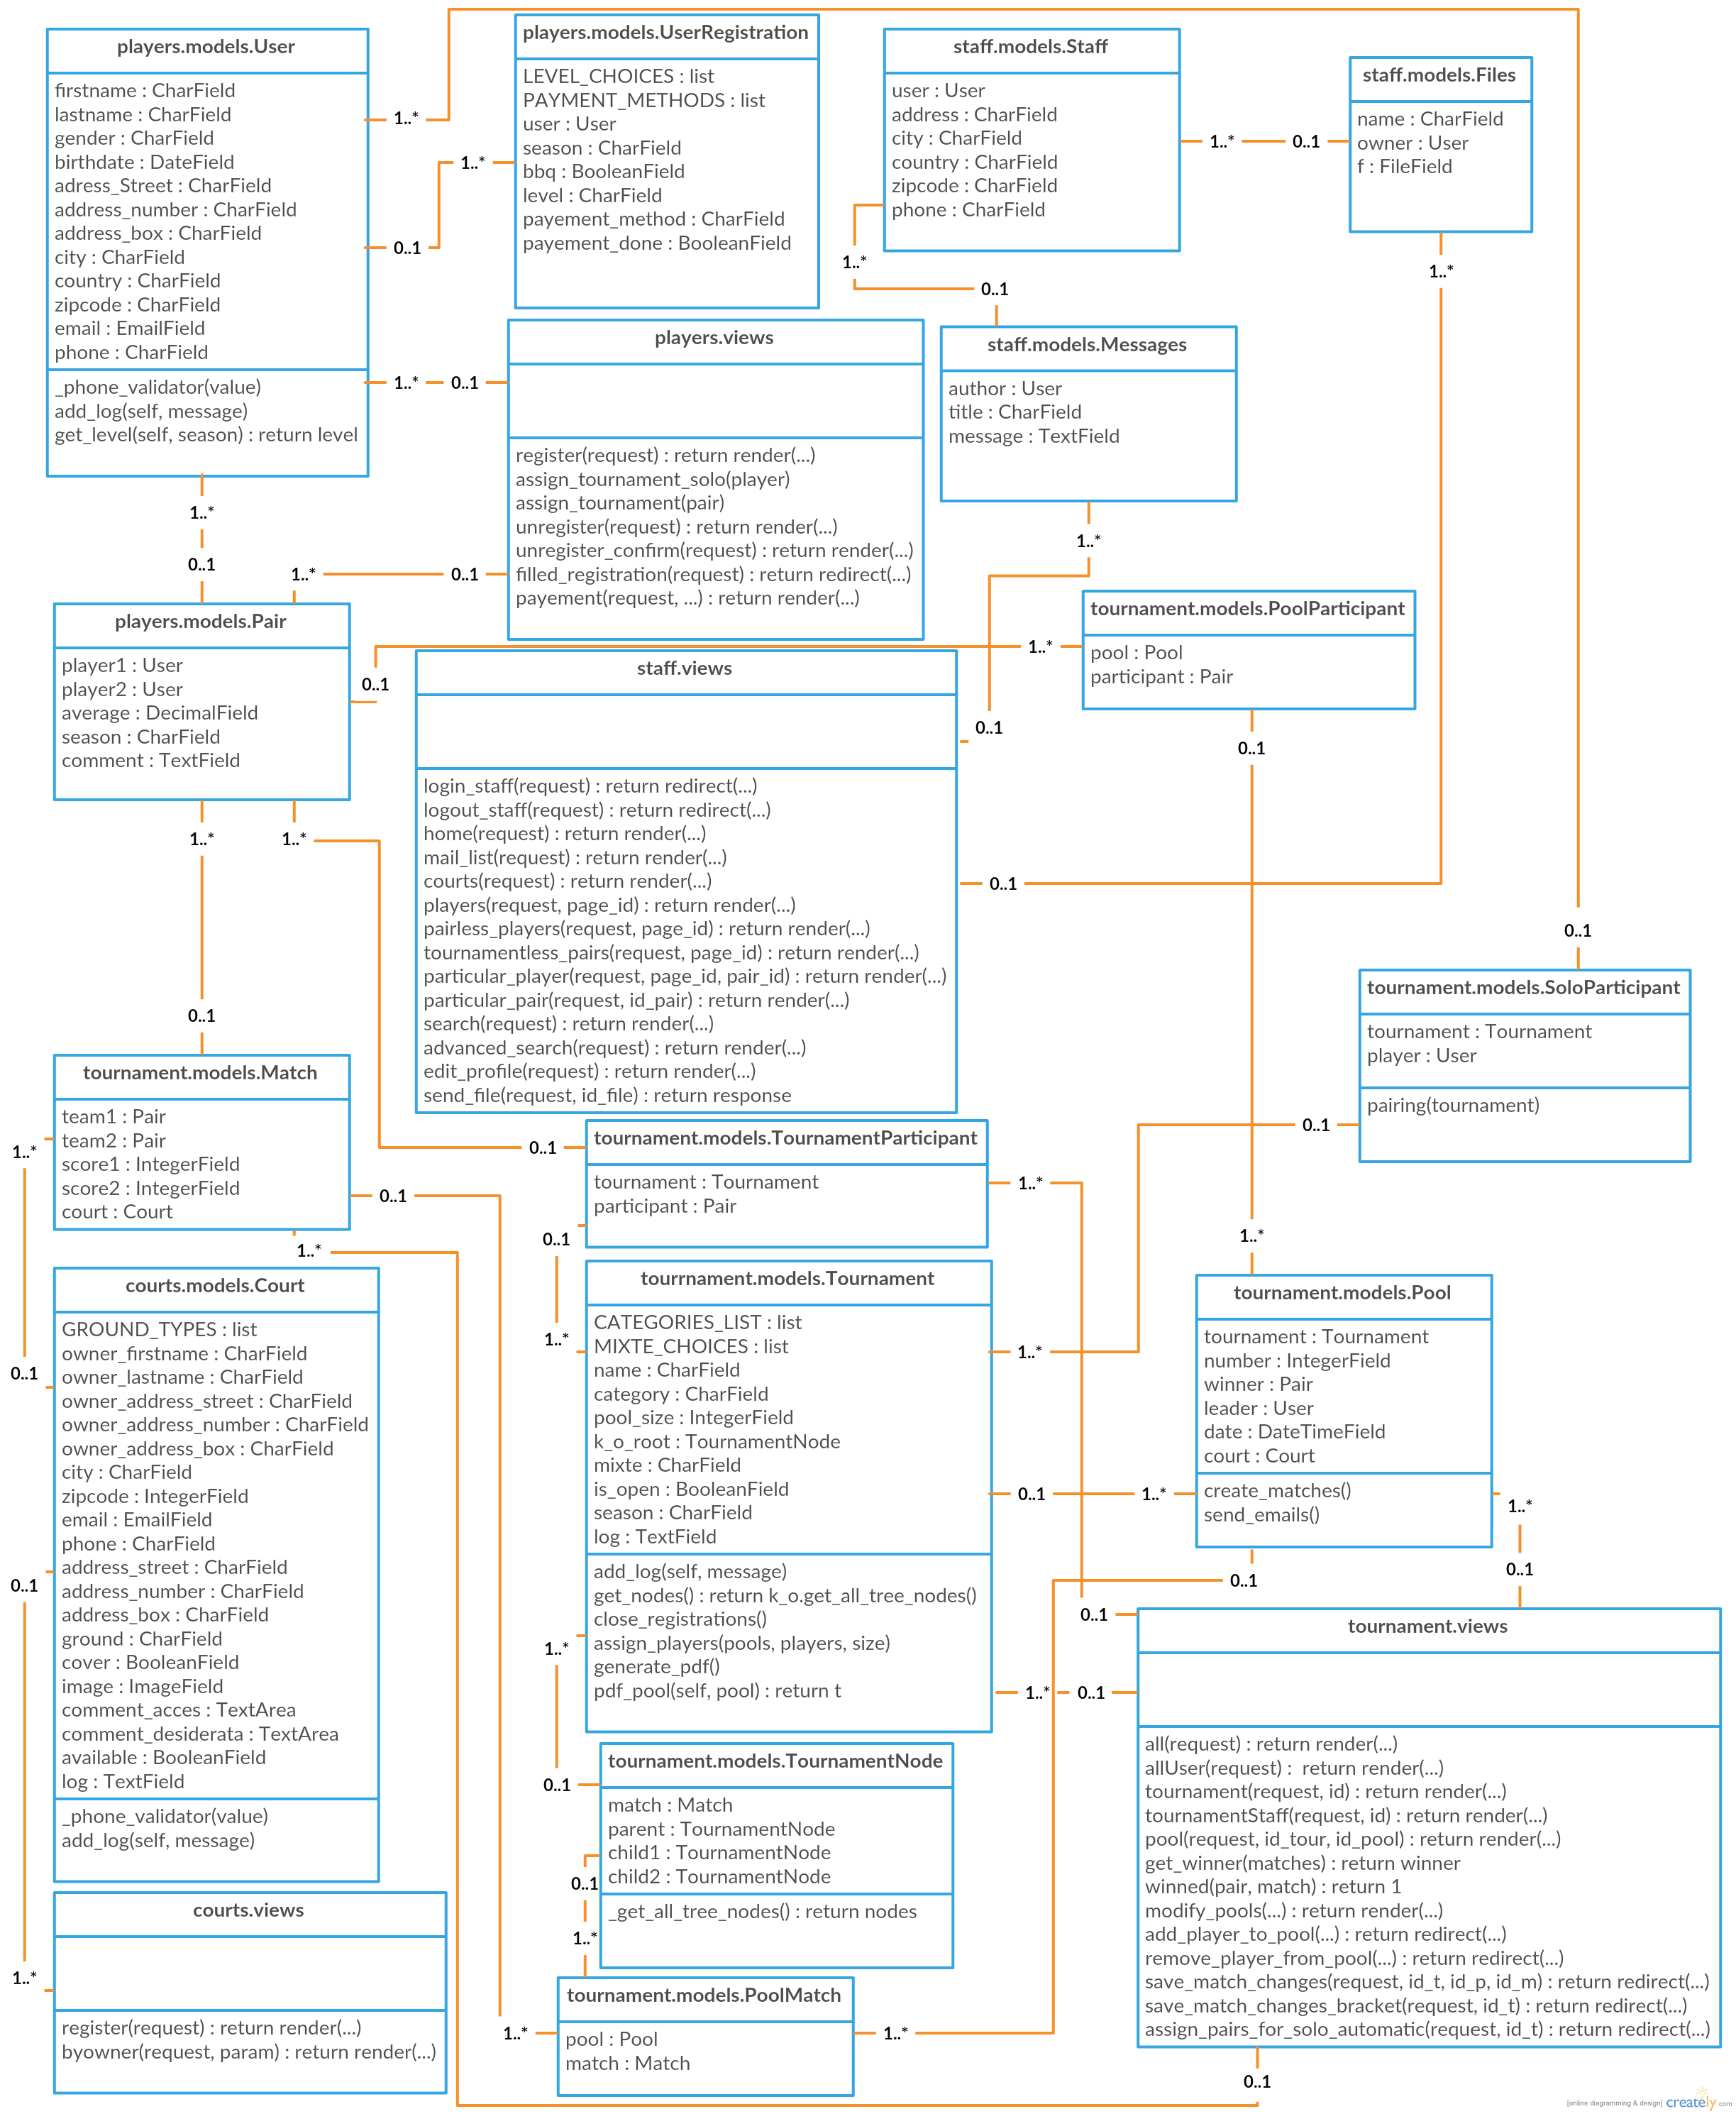
\includegraphics[scale=0.45]{Class.png}
\end{figure}

\subsection*{Sequences diagram}

You can see in figure \ref{sequence} the sequence diagram for how a player registers to a tournament with an email confirmation. Note that this is a registration for a single player. For two players, it works the same way but it creates a pair instead. 

%AJOUTER SEQUENCE ICI ET ENLEVER LES %, AJUTER LE SCALE EN FONCTION
\begin{figure}[position]
   \caption{\label{sequence} Sequence diagram}
   \includegraphics[scale=0.4]{sequence.png}
\end{figure}

\section{Conclusion}

For this phase, we took your feedback into account. All the must have requirements are now implemented, we will from now on focus on the design of the website, and polish the functionalities to make them run better and so that at the end of next phase we have a finale product. 

\end{document}